 \begin{center}
    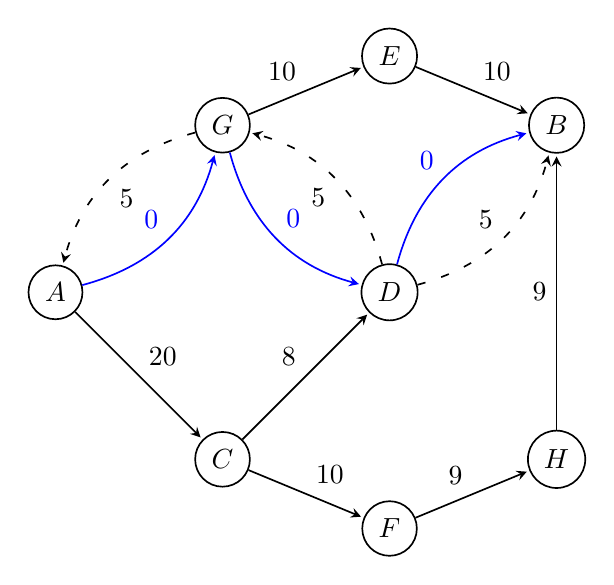
\begin{tikzpicture}[
            thick, 
            main/.style = {draw, circle}, 
            > = stealth, % arrow head style
            shorten > = 1pt, % don't touch arrow head to node
            auto,
            node distance = 3cm, % distance between nodes
            semithick % line style
        ]
        \node[main] (a) {$A$};
        \node[main] (g) [above right of=a] {$G$};
        \node[main] (c) [below right of=a] {$C$}; 
        \node[main] (d) [below right of=g] {$D$};
        \node[main] (e) [above of=d] {$E$};
        \node[main] (f) [below of=d] {$F$};
        \node[main] (b) [above right of=d] {$B$};
        \node[main] (h) [below right of=d] {$H$};

        \path[blue,->] (a) edge[bend right] node {0} (g);
        \path[->] (a) edge node {20} (c);
        \path[->] (c) edge node {10} (f);
        \path[->] (c) edge node {8} (d);
        \path[->, blue] (g) edge[bend right] node {0} (d);
        \path[->] (g) edge node {10} (e);
        \path[->] (e) edge node {10} (b);
        \path[->, blue] (d) edge[bend left] node {0} (b);
        \path[->] (f) edge node {9} (h);
        \path[->] (h) edge node {9} (b);
        
        \path[->, loosely dashed] (g) edge[bend right] node {5} (a);
        \path[->, loosely dashed] (d) edge[bend right] node {5} (g);
        \path[->, loosely dashed] (d) edge[bend right] node {5} (b);
    \end{tikzpicture} 
\end{center}